\part{Guide}
\begin{figure}[h]
    \centering
    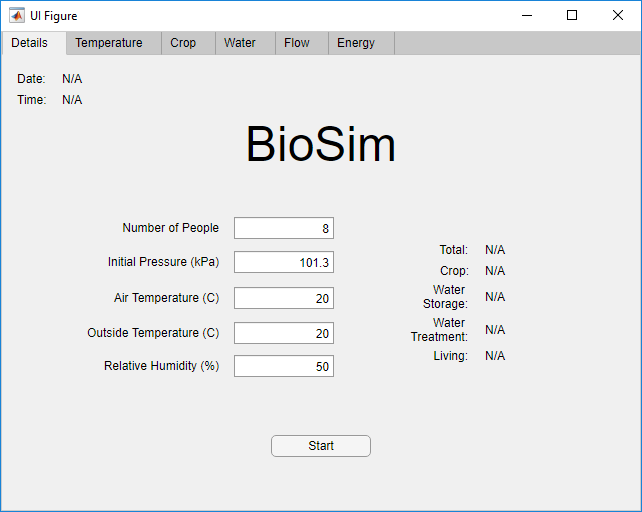
\includegraphics[width=0.6\textwidth]{guide_start}
    \caption{Start Page}
    \label{fig:guide_start}
\end{figure}
To begin, BioSim requires a few initial parameters (Figure \ref{fig:guide_start}). These parameters determine the required area for crop growth, water treatment, and living space. They also set parameters about the environment which will change how energy, water and air move throughout the system. 

\begin{figure}[h]
    \centering
    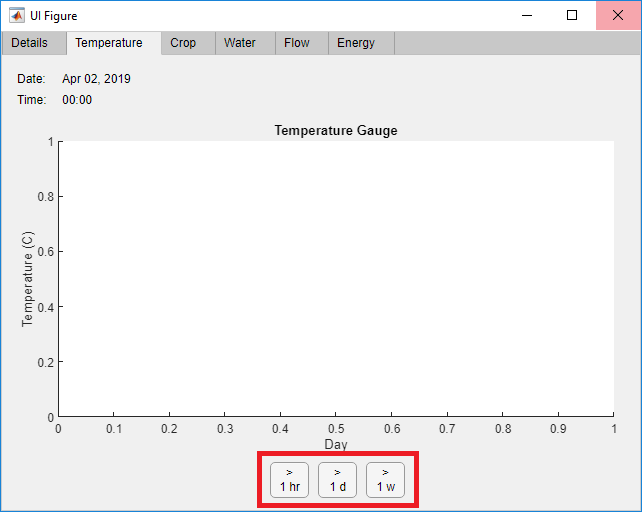
\includegraphics[width=0.6\textwidth]{guide_buttons}
    \caption{Time step buttons}
    \label{fig:guide_buttons}
\end{figure}

After clicking "Start", buttons will activate in the remaining tabs (Figure \ref{fig:guide_buttons}) which allow you to step the simulation for various time steps. A timer will also start in the upper left-hand corner which shows the current date and time.
\newpage

\begin{figure}[h]
    \centering
    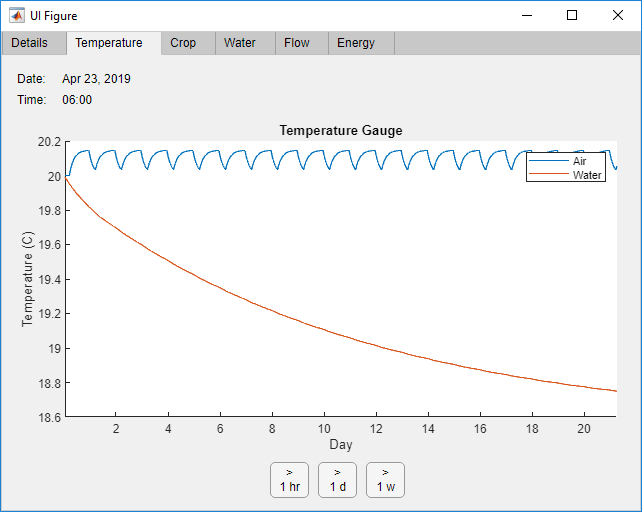
\includegraphics[width=0.65\textwidth]{guide_temp}
    \caption{Temperature Page}
    \label{fig:guide_temp}
\end{figure}

The Temperature tab (Figure \ref{fig:guide_temp}) shows the temperature of the air and water storage over time.


\begin{figure}[h]
    \centering
    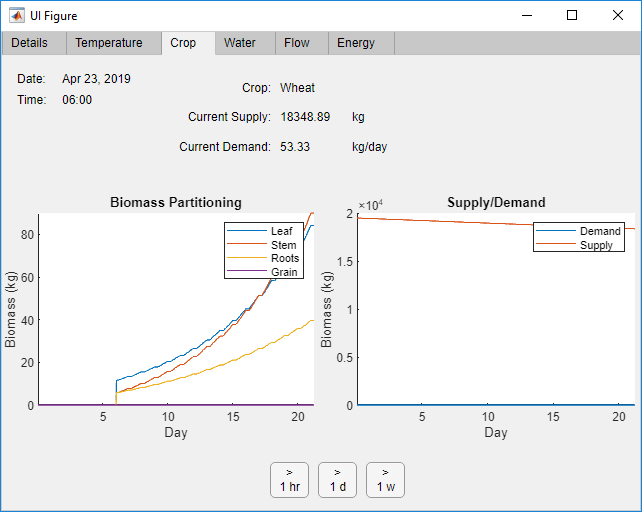
\includegraphics[width=0.65\textwidth]{guide_crop}
    \caption{Crop Page}
    \label{fig:guide_crop}
\end{figure}

The Crop tab (Figure \ref{fig:guide_crop}) shows the crop being grown, the amount in available supply, and the current demand. The graphs show the change in these values over time and how crop biomass partitions in the plants between leaves, stems, roots, and storage organs (grain).
\newpage

\begin{figure}[h]
    \centering
    \begin{subfigure}[h]{.47\textwidth}
        \centering
        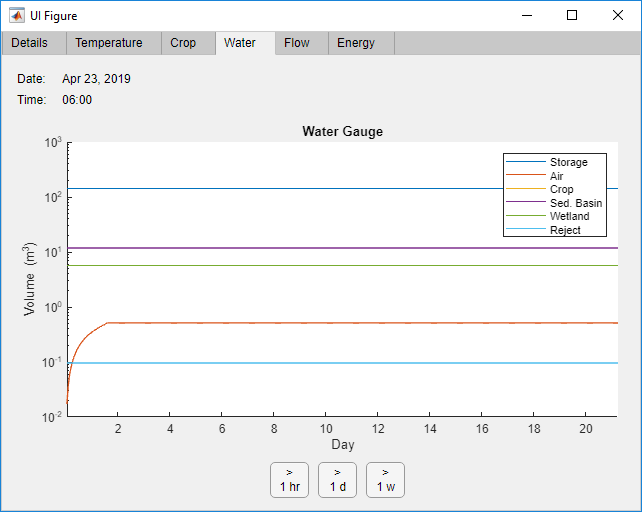
\includegraphics[width=\textwidth]{guide_water}
        \caption{Water Page}
        \label{fig:guide_water}
    \end{subfigure}
    \hfill
    \begin{subfigure}[h]{.47\textwidth}
        \centering
        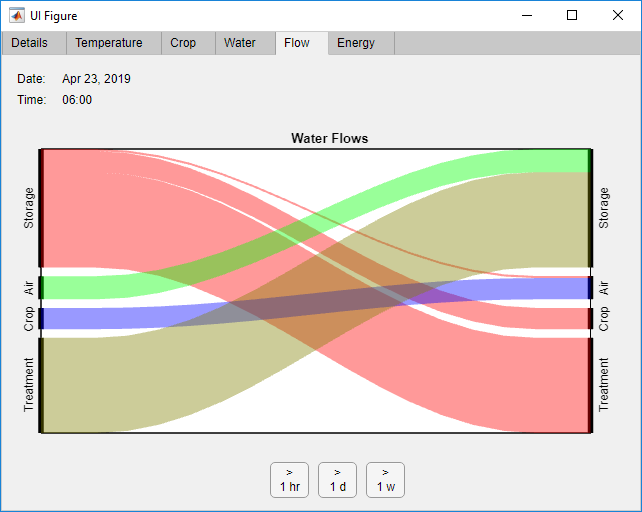
\includegraphics[width=\textwidth]{guide_flow}
        \caption{Flows Page}
        \label{fig:guide_flow}
    \end{subfigure}
\end{figure}

The Water tab (Figure \ref{fig:guide_water}) shows the distribution of water in the system. As everything is completely recycled, there is no net change in the total amount of water, only movement between different parts of the system. For this reason, the Flow tab (Figure \ref{fig:guide_flow}) shows the movement of water for the current hour.

\begin{figure}[h]
    \centering
    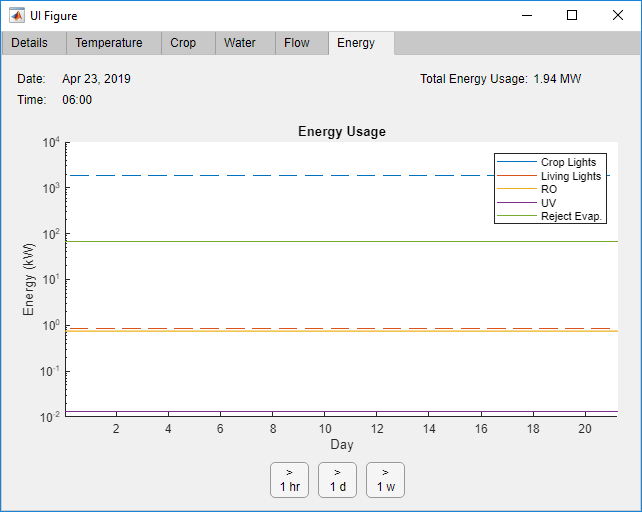
\includegraphics[width=0.65\textwidth]{guide_energy}
    \caption{Energy Page}
    \label{fig:guide_energy}
\end{figure}

Finally, the Energy tab (Figure \ref{fig:guide_energy}) shows the amount of energy consumption in different parts of the system on a logarithmic scale.